\documentclass{article}
\usepackage[utf8]{inputenc}
\usepackage{amstext}
\usepackage{amsmath} 
\usepackage{mathpazo}
\usepackage{graphicx} 
\usepackage{float} 
\usepackage{caption} 
\usepackage{epstopdf} 
\usepackage{hyperref}
\usepackage{varioref} 
\usepackage{fancyref}
\usepackage[section]{placeins} 
\usepackage{perpage}
\usepackage[margin=1in, paperwidth=8.5in, paperheight=11in]{geometry} 
\MakeSorted{figure} 
\usepackage{natbib}
\usepackage{graphicx}
\usepackage{xcolor}
\usepackage{listings}
\usepackage{minted}
\usepackage{subcaption}
\usepackage{eso-pic}
\usepackage{tikz}
\usepackage[american]{circuitikz}
\usepackage[font=small,labelfont=bf]{caption}

\title{ENGR2420 Lab 2 : Resistors and Diodes}
\author{Abigail Fry \\ Anusha Datar \\ Vienna Scheyer}
\date{February 20, 2019}

\begin{document}

\maketitle

\section{Experiment One : Diode-Connected Transistor Characteristics}
In this experiment we measured the current-voltage and voltage-current characteristics for a 2N3904 bipolar transistor using the circuits depicted in Figure \ref{fig:exp1}. From these circuits, we extracted the thermal voltage, saturation current, and incremental resistance of the diode-connected transistor.

When measuring the current-voltage characteristic, we chose to sweep from high currents to low currents to avoid dynamic artifacts of small currents causing charging/discharging in the wires used in the circuit. 

\begin{figure}[H]   
  \centering        
  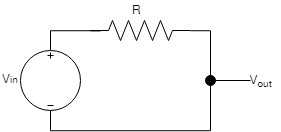
\includegraphics[scale = 0.5]{images/exp1_schematic.jpg}
  \caption{The circuits used to measure the voltage and the current across the transistor. The circuit on the left was used to measure voltage, and the circuit on the right was used to measure current.}   
  \label{fig:exp1}
\end{figure}

\subsection{Results}

\newline
\newline
The plot in Figure \ref{fig:plot1} contains the current-voltage characteristic, voltage-current characteristic, and a theoretical fit plotted on a voltage-current graph.  To generate the theoretical fit, we used MATLAB's polyfit function on the current-voltage characteristic data.  We then used that same theoretical line to find the values for the saturation current and thermal voltage based on the experimental data.
\begin{figure}[H]   
  \centering        
  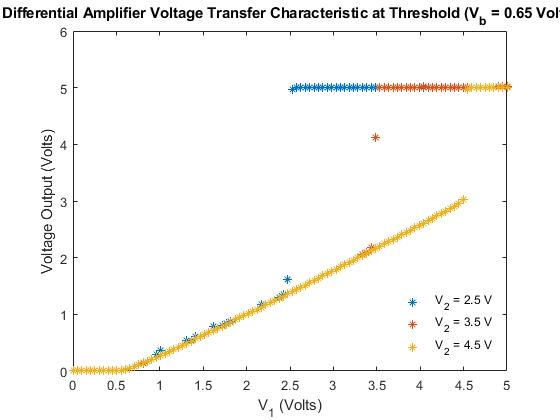
\includegraphics[scale = 0.5]{images/exp1_plot1.jpg}
  \caption{The current-voltage characteristic for the transistor. The current is plotted on a logarithmic scale on the y-axis.}   
  \label{fig:plot1}
\end{figure}

From our experimental results, we were able to extract values for the thermal voltage, $U_T$, and the saturation current, $I_s$. The experimental value for $U_T$ is 0.0269 Volts and the experimental value for $I_s$ is $1.2675$ x $ 10^{-15}$ Amps. 

The incremental resistance of the diode is associated with $\frac{\partial V}{\partial I}$. The log-log plot in Figure 3 shows the incremental resistance of the diode-connected transistor as a function of the current flowing through it as well as a theoretical fit of this.

\begin{figure}[H]   
  \centering        
  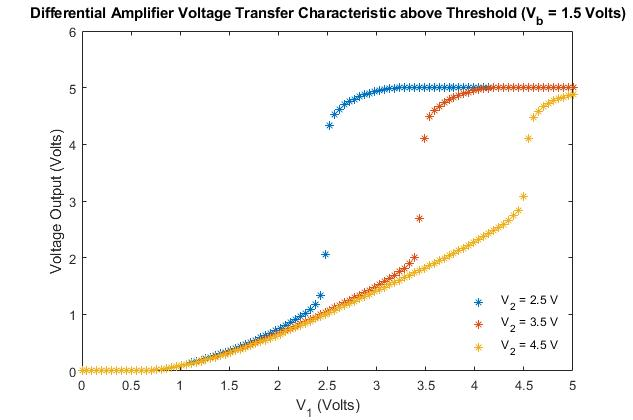
\includegraphics[scale = 0.5]{images/exp1_plot2.jpg}
  \caption{The incremental resistance of the diode as a function of the current flowing through it.}   
  \label{fig:inres}
\end{figure}

\subsection{Analysis}
We used the current-voltage equation from the prelab assignment to calculate the theoretical fit of the relationship between current and voltage for this circuit.
\begin{center}
    $I = I_s e^{\frac{V}{U_T}}$ \\
\end{center}
 
Then we re-arranged this equation to solve for voltage as a function of current for the voltage-current characteristic. 
 \begin{center}
     $V = U_T ln(\frac{I}{I_s})$
 \end{center}
 
To extract values for $U_T$ and $I_s$, we used linear regression (with the $polyfit$ function in MATLAB) to fit a line to the data using the voltage data points and the logarithm of the current data points for the current-voltage characteristic.  

As we showed in the prelab, we can manipulate the theoretical equation above into slope-intercept form to yield the following relationship: 

\begin{center}
    $ln(I) = \frac{1}{U_T} V + ln(I_s)$
\end{center}

Since we plotted our experimental data with the currents on the logarithmic axis, this slope-intercept equation relates linear voltage to logarithmic current. Therefore, the slope of the line returned by the $polyfit$ function is $\frac{1}{U_T}$ and the intercept is $ln(I_s)$. 

We used MATLAB's $polyfit$ function to fit a line to the measured current-voltage characteristic. The reason we used the current-voltage characteristic to calculate the theoretical parameters was that the voltage-current characteristic measurement had nonuniform behavior at low voltages, which was likely due to the limitations of the measurement equipment rather than the components themselves. Using the relationships we derived above, we determined that $U_T$ is 0.0269 Volts and $I_s$ is $1.2675$ x $10^{-15}$ Amps. Using these experimental parameters, we can create an exponential curve that characterizes the data with minimal deviations except for the low voltages on the voltage-current plot.  We included this theoretical plot in Figure 2.

After characterizing the current-voltage relationship, we calculated the incremental resistance of the diode-connected transistor as a function of the current flowing through it. To calculate the incremental resistance, we used MATLAB's \textt{diff} function on the  experimental input current and on the measured voltage from the current-voltage plot. Afterwards, we used Ohm's law to find the incremental resistance by finding the elementwise quotient of the two differentiated quantities. 
We calculated the theoretical incremental resistance for each measured current based on the relationship that we derived in the prelab:
$r_d = \frac{U_T}{I}$.
We graphed both of these values against our experimental input current, and our data points and the relationships between them are extremely consistent with each other. 

\subsection{Discussion}
There are substantial differences between the voltage-current and current-voltage characteristics along the voltage axis between 0.3 and 0.4 V.  The linear approximation fails to explain the data in this voltage range for the voltage-current characteristic.  The disparity between the current-voltage and voltage-current line may have come from the SMU's inability to measure the small current when there was a small input voltage.

As a whole, the exponential model fits the data well.  When plotted using MATLAB's $semilogy$ plotting feature, a linear approximation of voltage-current and current-voltage lines shows consistent behavior (on a $semilogy$ plot) that can be characterized with a first-order polynomial.

For incremental resistance, Figure \ref{fig:inres} shows the differences between the theoretical and experimental incremental resistance values. We found the theoretical and experimental incremental resistances in Ohms using the equations from the pre-lab and then plotted both on the same axes.  The variance between the theoretical and experimental values is minimal even though we used an element wise partial derivative for the experimental calculation and $r_d = \frac{U_T}{I}$ for the theoretical plot.  

\section{Experiment Two : Characteristics of a Resistor and Diode in Series}
This experiment involved placing three different resistors in series with a 2N3904 bipolar transistor as seen in the schematic in Figure 4. Placing the individual resistors in series allows us to evaluate the transition state behavior of the transistor in relation to the resistor values.  The resistor values spanned three orders of magnitude: 100 $\Omega$, 1K $\Omega$, and 10K $\Omega$. 
\begin{figure}[H]   
  \centering        
  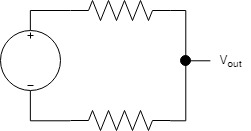
\includegraphics[scale = 0.5]{images/exp2_schematic.jpg}
  \caption{The circuits used to measure the voltage and the current across the transistor.}
  \label{fig:test4}
\end{figure}
With these circuits, we were able to measure the current-voltage and voltage-voltage responses of the system.

\subsection{Results}
When we generated the voltage-current characteristic, we also measured the voltage across the diode-connected transistor. From these values, we can create a voltage-voltage plot as seen in Figure \ref{fig:test5}.
\begin{figure}[H]   
  \centering        
  \includegraphics[scale = 0.5]{Volt-volt.png}
  \caption{The voltage-voltage plot for each resistor in series with the diode-connected transistor.}
  \label{fig:test5}
\end{figure}
This voltage-voltage plot shows that, when $V_{in}$ is lower than the $V_{on}$ voltage, the behavior of the transistor is linear. Using MATLAB's $polyfit$ tool, we determined that the slope of the line is about $0.9975$. Note that because this value is a ratio of voltage to voltage, it is dimensionless.


While conducting this measurement, we also measured the current through the circuit. We can compare the differences in the  voltage-current response for each resistor by plotting the input voltage against the logarithm of the current, as seen in Figure \ref{fig:test6}.  The moment where the line changes from linear to exponential behavior (from a semi-logrithimic point of view) is the transition moment for the 2N3904 bipolar transistor used in the lab.
\begin{figure}[H]   
  \centering        
  \includegraphics[scale = 0.5]{images/SVMI_semilog_allR.png}
  \caption{A plot on a a semilogy  plot showing input voltage vs output current for the 3 resistors in series with diode-connected transistor}
  \label{fig:test6}
\end{figure}
Then, to study each resistor's current response, we can create linear plots for each individual case as seen in Figure \ref{fig:test7}, Figure \ref{fig:test8}, and Figure \ref{fig:test9}. Each resistor's value differs by an order of magnitude. We plotted the data for each resistor value on separate plots to avoid obscuring the data due to the differing orders of magnitude.
\begin{figure}[H]   
  \centering        
  \includegraphics[scale = 0.5]{images/SVMI_Linear_100.png}
  \caption{A linear plot of the voltage response of the 100 Ohm resistor in series with the diode-connected transistor.}
  \label{fig:test7}
\end{figure}
\begin{figure}[H]   
  \centering        
  \includegraphics[scale = 0.5]{images/SVMI_Linear_1K.png}
  \caption{A linear plot of the voltage response of the 1K Ohm resistor in series with the diode-connected transistor.}
  \label{fig:test8}
\end{figure}
\begin{figure}[H]   
  \centering        
  \includegraphics[scale = 0.5]{images/SVMI_Linear_10K.png}
  \caption{A linear plot of the voltage response of the 10K Ohm resistor in series with the diode-connected transistor.}
  \label{fig:test9}
\end{figure}

We were then able to extract the $I_{on}$ and $V_{on}$ values for each resistor-transistor combination and plot those values as a function of the value of the resistor. 
\begin{figure}[H]   
  \centering        
  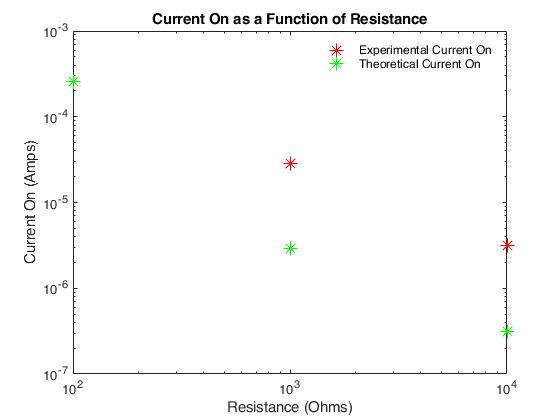
\includegraphics[scale = 0.5]{images/curr_res.jpg}
  \caption{A plot of the turn-on current of the resistor-diode connected transistor series combination as a function of the resistor value.}
  \label{fig:test10}
\end{figure}
\begin{figure}[H]   
  \centering        
  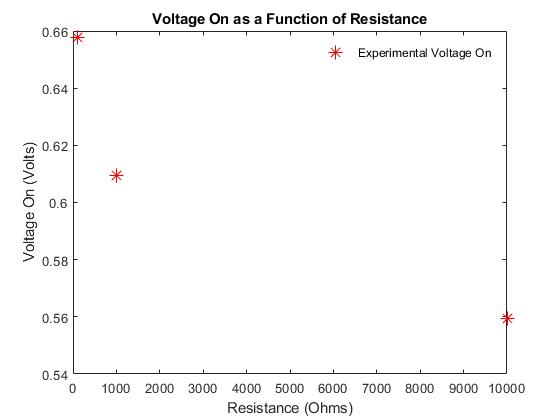
\includegraphics[scale = 0.5]{images/vol_res.jpg}
  \caption{A plot of the turn-on current of the resistor-diode connected transistor series combination as a function of the resistor value.}
  \label{fig:test11}
\end{figure}
\subsection{Analysis}
% Plot 1: Voltage-Voltage
To create the voltage-voltage plot, we measured the voltage across the transistor while actively supplying voltage. This voltage-voltage plot shows that, when $V_{in}$ is lower than the $V_{on}$ voltage, the behavior of the transistor is linear. Using MATLAB's $polyfit$ tool, we determined that the slope of the line is about $0.9975$. This value has no unit because it is a ratio between two quantities of the same units. Theoretical expectations align with this experimental slope. Since the voltage is below the threshold dictated by $V_{on}$, the input voltage should be roughly equal to the output voltage, which would require a 1:1 ratio. 
Therefore, the error associated with this experiment is $\frac{1 - 0.9975}{1} = 0.0025$, or .25\%.
\newline
\newline
% Plot 2 : Current-Voltage Semilog
For the current-voltage plot, we observed an exponential relationship between current and voltage at low voltages and then a linear relationship between current and voltage at high voltages. On the semilogarithmic axes, this translates to a linear relationship at low voltages and a gradually increasing curve at higher voltages. As the resistor value increases, the line is steeper, and the total current output at a given voltage is slightly higher.
This experimental data reflects theoretical expectations; at lower voltages, the value should reflect the mainly exponential relationship where $I$ is proportional to $\frac{1}{I_s}e^{\frac{V_{in}}{U_T}}$. To generate the theoretical plot, we used MATLAB's $polyfit$ function and the procedure described in Experiment One to find the values of $U_T$ and $I_s$. 
While the shape of the experimental plot generally matches the exponential fit that we expected, there are some deviations. This is most likely due to the fact that the slope of the line is quite steep at low voltages on semilog axes so the line has a lower density of data points. Additionally, some of these points are at such low currents that the data is effectively useless (since the SMU cannot measure extremely low values of current). This caused some challenges with fitting lines to the data, but even so these fits are fairly accurate. In the future, we may want to consider collecting a higher density of data points at the beginning.
\newline 
\newline
% Plots 3-5 : Current-Voltage Linear individuals
While the current-voltage plots on semilogarithmic axes allow us to examine the exponential behavior of the diode-connected transistor, the individual plot on linear axes allow us to consider the linear behavior of the resistor. In this case, when $V_{in}$ is greater than $V_{on}$, the circuit follows Ohm's law, $V=IR$. Therefore, as the value of the resistor increases by an order of magnitude, the slope increases by an order of magnitude as well. The straight line plots in Figures 7, 8, and 9 reflect this theoretical relationship. By creating individual plots for each resistor, we could individually examine this relationship for each resistor value.
\newline
\newline
% Plot 6 : Ion
The plot of the turn-on currents of the diode connected transistor as a function of the series resistance reflects an inversely proportional relationship between $I_{on}$ and $R$. This matches theoretical expectations because, as proven in the prelab assignment, $I_{on} = \frac{U_T}{R}$. 
\newline
\newline
% Plot 7 : Von
The plot of the turn-on voltages of the diode connected transistor as a function of the series resistance shows an inversely proportional, exponentially decaying relationship between $V_{on}$ and $R$. This reflects theoretical expectations because, as proven in the prelab assignment, $V_{on} = U_{T}log(\frac{U_{T}}{RI_{s}})$. Both the experimental values and theoretical frameworks display similar behavior.
\subsection{Discussion}
The plots above show that the experimental data matches the expected theoretical behavior of our circuit. The data plotted in Figure \ref{fig:test5} and Figure \ref{fig:test6} allows us to analyze the behavior of the circuit before the transitional moment, $V_{on}$. On semilogarithmic axes, this region before $V_{on}$ appears linear.
The plots in Figures \ref{fig:test7}, \ref{fig:test8}, and \ref{fig:test9} show the behaviour of the circuit after $V_{on}$. In this region of the data, the linear axes show that the circuit behavior is mainly determined by the resistor. Here, the transistor acts as a diode and the resistor is the main component acting in the circuit.

$V_{on}$ and $I_{on}$ vary with respect to $R$ as expected from our pre-lab analysis.  The equation derived in the pre-lab for  $I_{on}$ was $I_{on} =\frac{U_{T}}{R}$.  The expected decay of $I_{on}$ as $R$ increases is seen in Figure \ref{fig:test10}.  The equation derived in pre-lab is  $V_{on} = U_{T}log(\frac{U_{T}}{RI_{s}})$.  As $R$ increases, $V_{on}$ decays as expected as seen in Figure \ref{fig:test11}.
\end{document}
